\documentclass[tikz]{standalone}
\usepackage{pgfplots}
\usepackage{xcolor}
\usetikzlibrary{calc}
\definecolor{mycolor}{HTML}{888888}
\pgfplotsset{compat=1.18}

\begin{document}
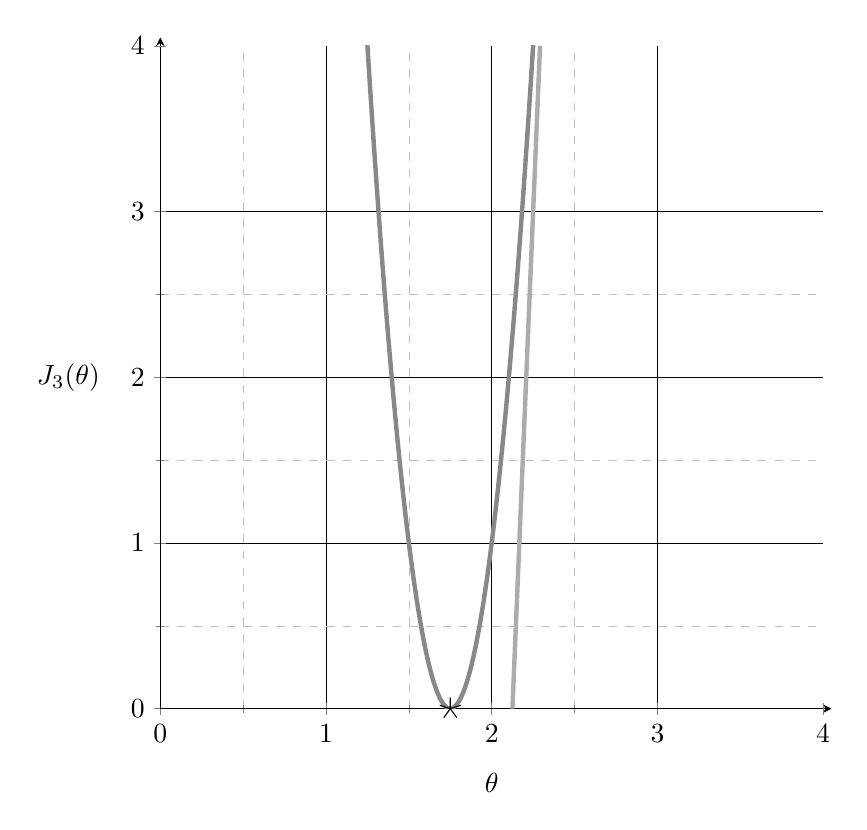
\begin{tikzpicture}
  \begin{axis}[
    axis lines=left,
    x axis line style={->,>=stealth, shorten >=-3pt},
    y axis line style={->,>=stealth, shorten >=-3pt},
    xlabel={\(\theta\)},
    ylabel={\(J_3(\theta)\)},
    ylabel style={rotate=-90},
    xmin=0, xmax=4,
    ymin=0, ymax=4,
    xtick={0,1,...,3},
    ytick={0,1,...,3},
    extra x ticks={4},
    extra x tick style={grid=none},
    extra y ticks={4},
    extra y tick style={grid=none},
    minor x tick num=1,
    minor y tick num=1,
    grid=both,
    major grid style={line width=0.2pt,draw=black},
    minor grid style={line width=0.1pt,draw=gray!50,dashed},
    width=10cm,
    height=10cm,
  ]
    % Plot the single error term (without 1/3): (4θ-7)^2
    \addplot[domain=0:4, samples=200, ultra thick, color=mycolor]
      {(4*x-7)^2};

    % Mark the minimum at θ=7/4=1.75
    \addplot[only marks, mark=star, mark options={scale=2, fill=red}] 
    coordinates {(1.75,0)};
    % Tangent line at θ=2.5: y = 24(x-2.5)+9, clipped to visible y∈[0,4]
    % Visible segment occurs for x ∈ [2.125, 2.2916667]
    \addplot[domain=2.125:2.2916667, samples=2, ultra thick, color=mycolor!70]
      {24*(x-2.5)+9};
  \end{axis}
\end{tikzpicture}
\end{document}


